\problemname{Lög um lög}
\illustration{0.3}{music}{Mynd fengin af \href{https://www.flickr.com/photos/186095195@N02/49395693758}{flickr.com}}

Það tíðkast mikið í popptónlist, og kemur einnig fyrir í annarri tónlist, að vinsælustu lögin fylgi sama hljómagang.
Það veitir hlustendum kunnugleika um leið, og því líklegt að þeim líki við lagið.
Þetta getur samt skapað vandamál þegar kemur að höfundarétti.
Þar sem hljómagangur er oft sá sami er takmarkaður fjöldi laglína, eða nóturnar sem eru sungnar, sem geta komið til greina.
Því hefur gerst að lögsóknir spretti upp þar sem lagahöfundur er ásakaður um ritstuld.
Ástæðan er þá sú að hluti laglínu í einu lagi hljómar nákvæmlega eins og hluti laglínu í öðru lagi.

Til dæmis var Katy Perry lögsótt af Marcus Gray vegna lagsins Dark Horse.
Upprunalega var dæmt í hag Marcus Gray en seinna var því snúið við því partur laglínunnar sem var vísað í var ekki sérstaklega einstakur eða sjaldgæfur.
Það er nefnilega hættulegt að setja fordæmi fyrir að hver sem er geti lögsótt hvern sem er fyrir örfáar nótur.
Þess vegna þarf þetta oftast að vera nægilega stór hluti lagsins, ekki bara nokkrar sekúndur.
Af og til kemur upp að laglínur tveggja laga séu alveg eins yfir langan tíma og þá er trúin sú að ritstuldur hafi átt sér stað.
Auðvitað er mögulegt að það komi upp fyrir tilviljun. 
Það gerist því sérstök stærðfræði er á bakvið hvaða tónar hljóma vel á eftir hvorum öðrum, sem tónskáld annaðhvort kunna eða hafa innsæi fyrir.

Nú hefur plötuútgefandi áhyggjur af því að verið sé að brjóta á höfundarétti sínum.
Það tekur of langan tíma að hlusta á öll lögin sem gætu verið eins þannig plötuútgefandinn hefur samband við þig.
Beðið er um að útfæra forrit sem getur greint tvö lög samtímis, annað frá plötuútgefandanum og hitt frá meinta höfundarréttaþjófinum.
Forritið á að ákvarða hvort lögin séu nógu lík til þess að lögsókn eigi rétt á sér.
Þessi plötuútgefandi hefur miklar áhyggjur af því að höfða lögsókn sem yrði dæmd í hag verjandans og vill því bara lögsækja ef lögin eru
í heild sinni eins, með tilliti til tónfræðinnar.

Hver \emph{nóta}, eða tónn, hefur sína tíðni. Nóg er að ákveða tíðni einnar nótu og þá má reikna tíðni hinna nótnanna út samkvæmt reglu.
\emph{Áttund} er skilgreind sem bil milli tveggja nótna þar sem önnur nótan er með tvöfalda tíðni hinnar nótunnar.
Í hefðbundinni Evrópskri tónlist er oftast skipt áttundinni í tólf tíðnir sem koma í röð, sem nefnast krómatíski skalinn,
með jafnstór bil milli hverrar nótu á eftir annarri, sem nefnist \emph{hálftónsbil}.
\emph{Heiltónsbil} er því tvö hálftónsbil.
Á píanói má sjá þessa tólf tóna, og koma þeir oft fyrir, eitt skipti í hverri áttund, en oftast með ókláruðum áttundum lengst til hægri og lengst til vinstri.

\begin{figure}[ht!]
  \centering
    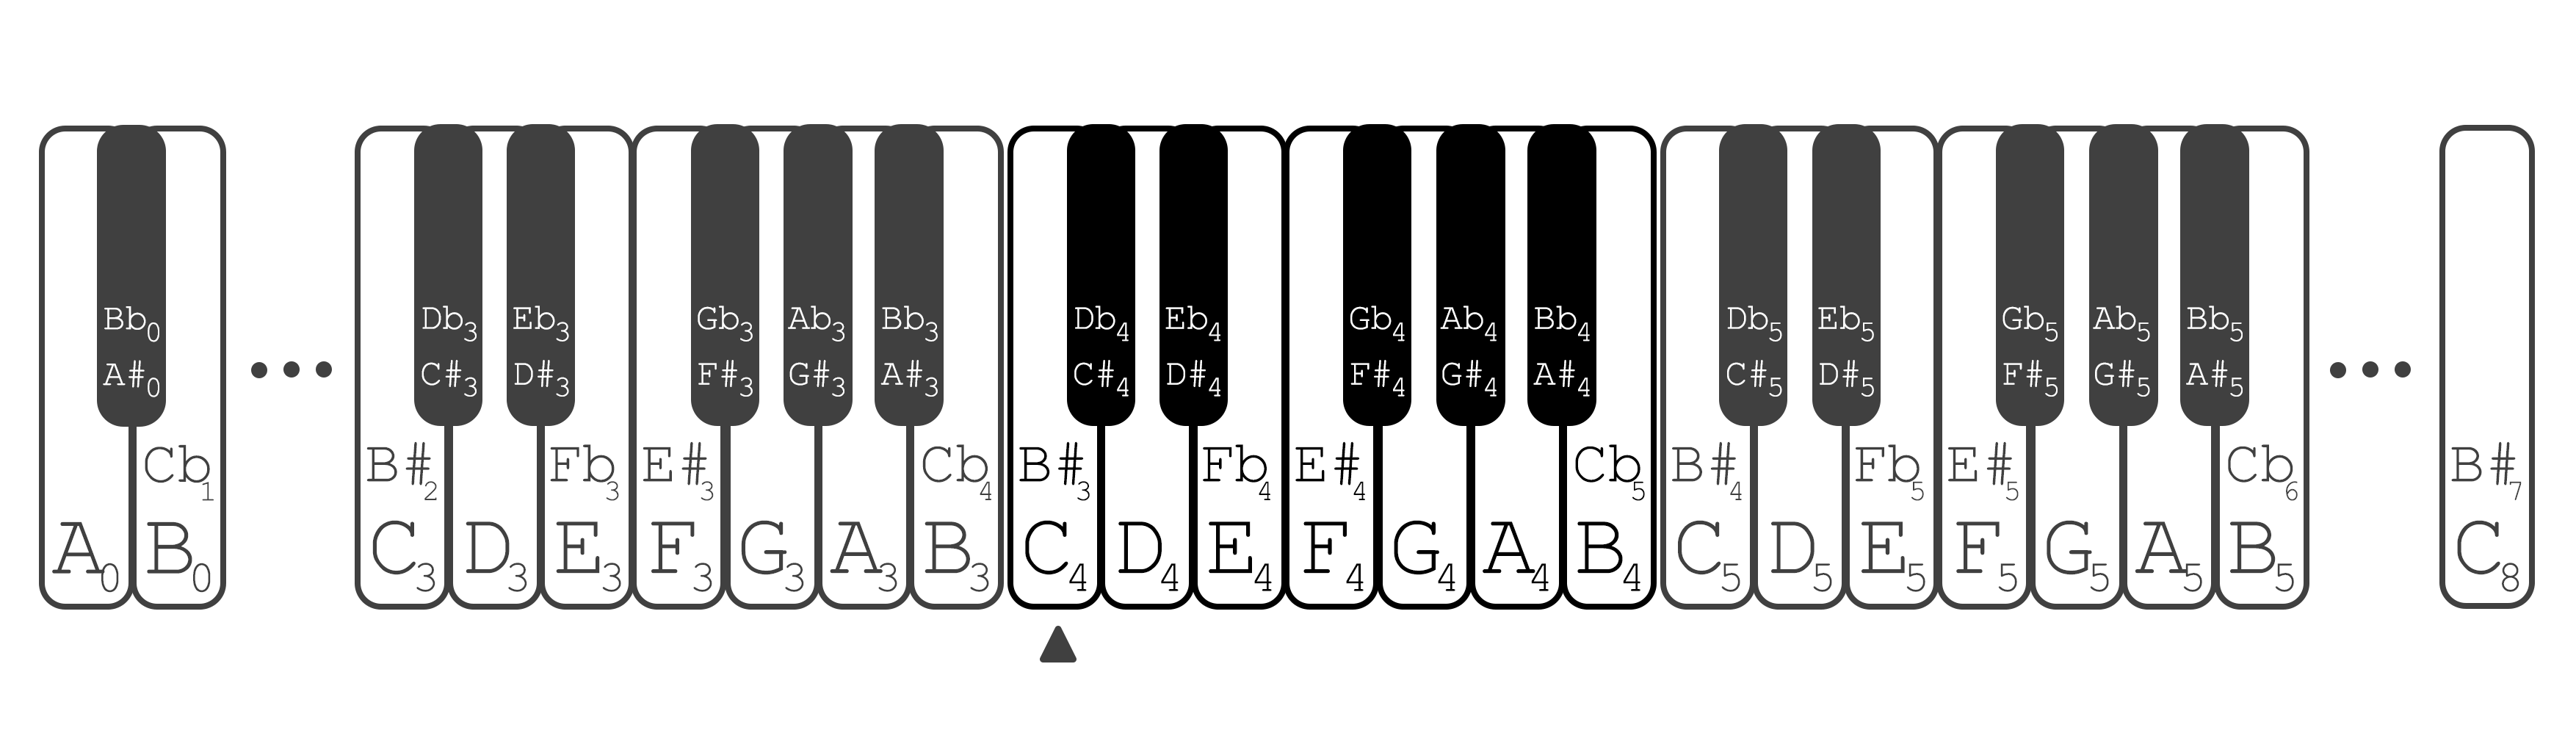
\includegraphics[width=0.9\textwidth]{piano}
  \caption{Nótur merktar á lyklum píanós.}
\end{figure}

Píanó eru byggð með sjö tóna dúr skalann í huga, þá sérstaklega \texttt{C} dúr.
Þá er grunnnótan \texttt{C} og skalinn fylgir formúlunni:
heiltónsbil, heiltónsbil, hálftónsbil, heiltónsbil, heiltónsbil, heiltónsbil, hálftónsbil.
Nóturnar eru nefndar eftir bókstöfunum \texttt{A-G} eins og má sjá á myndinni og samanstendur \texttt{C} dúr skalinn af nótunum \texttt{C D E F G A B}, og samsvara þær hvítu lyklunum á píanóinu.
Nóturnar sem eru ekki í \texttt{C} dúr eru nákvæmlega þær sem samsvara svörtu lyklunum á píanói.
Þær eru nefndar út frá hinum nótunum með hálftónshækkunum eða hálftónslækkunum.
Hálftónshækkun er rituð með því að bæta við \texttt{\#} á eftir nótunni, en hálftónslækkun er rituð með því að bæta við \texttt{b} á eftir nótunni.
Því eru nóturnar í einni áttund \texttt{C C\#/Db D D\#/Eb E F F\#/Gb G G\#/Ab A A\#/Bb B}, en athugið einnig að \texttt{Cb} samsvarar \texttt{B}, \texttt{B\#} samsvarar \texttt{C}, \texttt{Fb} samsvarar \texttt{E} og \texttt{E\#} samsvarar \texttt{F}
Til að merkja á hvaða áttund er verið að spila er notast við heiltölur, sem er bætt við aftast á hverja nótu fyrir sig.
Áttundirnar eru í hækkandi röð frá vinstri til hægri á píanói og merkir fyrsta \texttt{C} nótan byrjun áttundar númer $1$.
Ef fjórða áttundin væri skrifuð upp mætti skrifa hana sem \texttt{C4 C\#4 D4 D\#4 E4 F4 F\#4 G4 G\#4 A4 A\#4 B4}.
Nótan sem er lengst til vinstri á $88$ lykla píanói er \texttt{A0}, nótan sem er þekkt sem miðju \texttt{C} er \texttt{C4}, merkt með þríhyrningi á myndinni, og nótan lengst til hægri er \texttt{C8}.

Laglínur eru stór partur af lögum og má skilgreina þær sem runu af nótum og þögnum.
Þagnir eru táknaðar með \texttt{-} og tákna að ekki sé spilað nótu.
Hver nóta eða þögn endist í jafn langan tíma.
Hægt er að ákvarða hvort að tvö lög séu eins eftir ákveðnum reglum:

\begin{itemize}
  \item Regla 1: Ef tvær laglínur eru ritaðar nákvæmlega eins að þá tákna þær sama lagið.
  Til dæmis eru \texttt{C4 D4 - E4} og \texttt{C4 D4 - E4} eins.
  \item Regla 2: Ef tvær laglínur eru ritaðar á mismunandi máta, en nóturnar eru hinar sömu að þá tákna þær sama lagið.
  Til dæmis eru \texttt{C4 C\#4 - Eb4} og \texttt{B\#3 Db4 - D\#4} eins.
  \item Regla 3: Ef tvær laglínur eru ritaðar eins, nema öllum nótunum í annarri þeirra hefur verið hliðrað um sama fjölda áttunda að þá tákna þær sama lagið.
  Til dæmis eru \texttt{B3 D4 - E4} og \texttt{B5 D6 - E6} eins.
  \item Regla 4: Ef tvær laglínur eru ritaðar eins, nema öllum nótunum í annarri þeirra hefur verið hliðrað um sama fjölda hálftóna að þá tákna þær sama lagið.
  Til dæmis eru \texttt{B3 D4 - E4} og \texttt{C\#4 E4 - F\#4} eins.
\end{itemize}

Ef ekki hefur verið ákvarðað að lögin séu eins eftir notkun þessarra reglna að þá eru lögin ekki eins.

\section*{Inntak}
Inntak byrjar á einni línu með einni jákvæðri heiltölu $n$, þar sem $1 \leq n \leq 10^5$, sem tákna lengdir laglínanna.
Næst koma tvær línur, hvor með einni laglínu fyrir sig, þar sem laglínunnar innihalda $n$ gildi sem tákna ýmist nótur eða þagnir, aðskilnar með bilum.
Nótur og þagnir eru ritaðar á sama formi og var lýst fyrr í lýsingunni.
Lægsta nótan sem getur komið fyrir í inntaki er \texttt{A0} og hæsta nótan er \texttt{C8}, sem samsvarar $88$ lykla píanói.
Sérhver nóta inniheldur mesta lagi eitt \texttt{\#} tákn eða \texttt{b} tákn.


\section*{Úttak}
Skrifaðu út \texttt{Jebb} ef lögin eru eins og plötuútgefandinn á að lögsækja, annars skaltu skrifa út \texttt{Neibb}.

\section*{Stigagjöf}
\begin{tabular}{|l|l|l|}
\hline
Hópur & Stig & Takmarkanir \\ \hline
1     & 15   & Nota þarf reglu $1$ \\ \hline
2     & 25   & Nota þarf reglur $1$ og $2$ \\ \hline
3     & 15   & Nota þarf reglur $1$ og $3$ \\ \hline
4     & 10   & Nota þarf reglur $1$, $2$ og $3$ \\ \hline
5     & 35   & Nota þarf allar reglur \\ \hline
\end{tabular}

\section*{Auka um sýnidæmi}
Til að hlusta á laglínurnar í sýnidæmunum getið þið náð í hljóðskrár \href{/problems/iceland.logumlog/file/statement/attachments/melodies.zip}{hér}.
Í sýnidæmi $5$ má heyra parta af laglínum laganna Ég Á Líf eftir Örlyg Smára, fyrri laglínan, og I Am Cow eftir hljómsveitina The Arrogant Worms, seinni laglínan.
Í sýnidæmi $8$ má heyra tvo parta af laglínu lagsins Paradise Lost eftir Symphony X, þar sem seinni laglínan er sú sama og fyrri, nema hækkuð upp um heiltónsbil.
